\begin{document}

\section{ユーザインタフェース設計}
本システムの画面の詳細及び画面遷移について説明する.使用している画像において,指定がない場合以外は赤色の部分がキーボード入力を行う場所,黄色の部分がクリックを行う場所である.
\subsection{画面遷移図}
付録Bにて画面遷移図を記載.
\subsection{ログイン・総合TOP画面}

\subsubsection{ログイン画面}
図\ref{fig:login1}にログイン画面を示す.

\begin{figure}[H]
    \begin{minipage}{0.5\hsize}
        \centering
        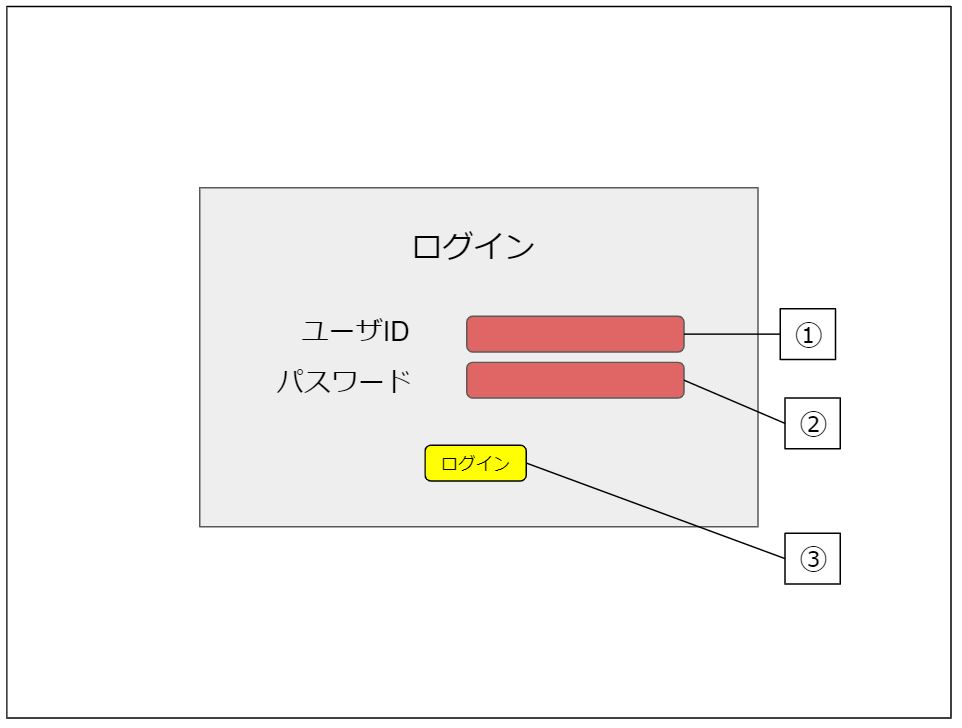
\includegraphics[width=7cm]{UI-umino/login1.JPG}
        \caption{ログイン画面}
        \label{fig:login1}
    \end{minipage}
    \begin{minipage}{0.5\hsize}
        \centering
        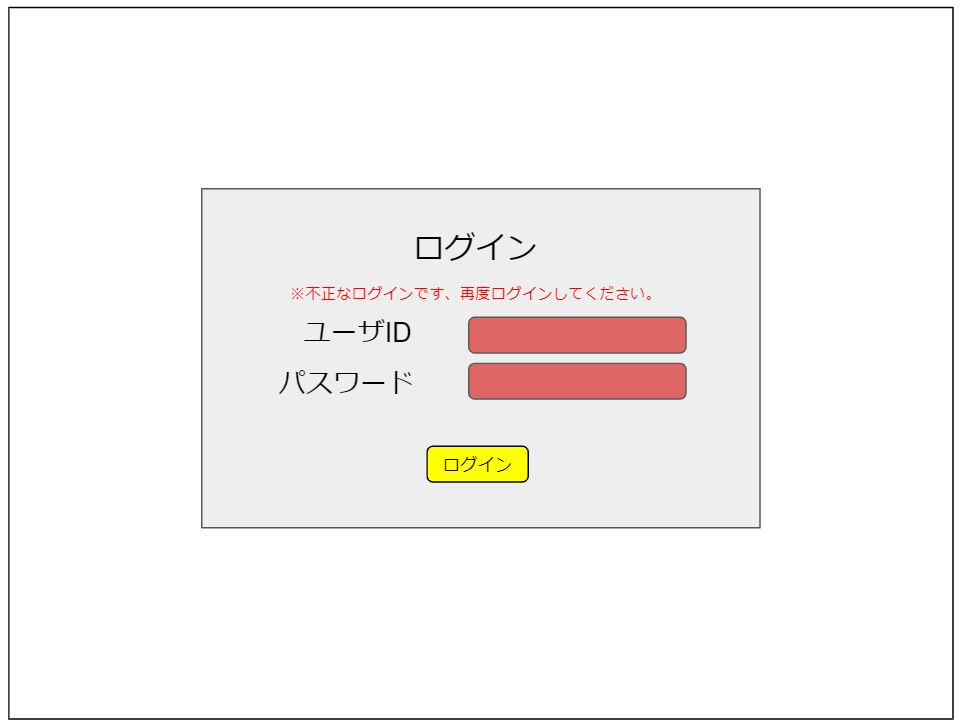
\includegraphics[width=7cm]{UI-umino/login2.JPG}
        \caption{再ログイン画面}
        \label{fig:login2}
    \end{minipage} 

\end{figure}

\begin{enumerate}
\renewcommand{\labelenumi}{\textcircled{\scriptsize \theenumi}}
\item ユーザID入力\\ ログインユーザは事前に設定しておいたログインIDを入力する.
\item パスワード入力\\ ログインIDと同じく,事前に設定しておいたパスワードを入力する.
\item ログイン\\ ログインをクリックすることで図\ref{fig:TOP1}に遷移する.ただし,ユーザIDに対応したパスワードが一致しない場合には図\ref{fig:login2}に遷移し,再入力を要求される.
\end{enumerate}

\subsubsection{総合TOP画面}
図\ref{fig:TOP1}に総合TOP画面を示す.総合TOP画面では,フロント業務,清掃業務,レストラン業務,マニュアル・質問閲覧,管理者専用機能をクリックすることでそれぞれの画面に遷移する.ログアウトをクリックした場合には,ログアウト処理がされ図\ref{fig:login1}に遷移する.

\begin{figure}[H]
 \centering
   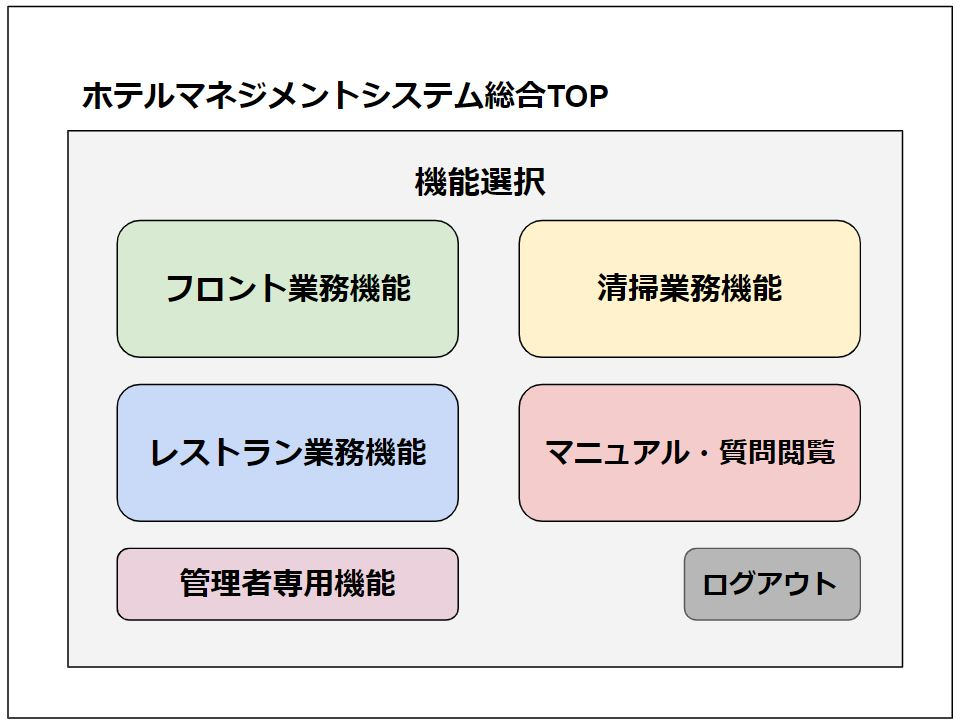
\includegraphics[width=100mm]{UI-umino/TOP1.JPG}
 \caption{総合TOP画面}
 \label{fig:TOP1}
\end{figure}

\end{document}